\section{Analysis tasks}\label{sec:analysis-tasks}

In this section, we study a gamut of fundamental analysis tasks, namely function reconstruction
(\autoref{sec:rmse-optimized}), derivative computation (\autoref{sec:gradient} and
\autoref{sec:laplacian}), histogram computation (\autoref{sec:histogram}), and isocontour extraction
(\autoref{sec:isocontour}). For each task, we define an error metric $e$ that is the basis for
evaluating performance of different streams on the task. We use Algorithm~\ref{alg:greedy} to
compute a stream $s_{opt}$ that is optimized for each task. An $s_{sig}$ stream is computed from the
signature of $s_{opt}$. We compare $s_{lvl}$, $s_{bit}$, $s_{wav}$, $s_{mag}$, $s_{sig}$, and
$s_{opt}$ by plotting the error as a function of the number of packets received. To mimic the
effects of entropy compression commonly used in practice, we remove all packets that contain only
leading zero bits from each stream, before plotting. This comparison is performed on a variety of
data sets, listed in \autoref{tbl:data-sets}.

\begin{table*}[t]
  \caption{Data sets used in experiments \duong{Update this table}}
  \centering
  \begin{tabular}{p{0.15\linewidth}p{0.20\linewidth}p{0.15\linewidth}p{0.10\linewidth}p{0.15\linewidth}}
  \hline
  Name & Source & Slice dimension & Type & Citation\\
  \hline
  boiler & combustion simulation& $140\times 148$ & float64 &\\
  euler & fluid simulation& $256\times 1024$ & float64 &\\
  kingsnake & CT scan & $1024\times 795$ & uint8 &\\
  plasma & magnetic reconnection simulation& $512\times 512$ & float32 &\\
  marschner-lobb & analytical function& $256\times 256$ & float64 &\\
  diffusivity & hydrodynamics simulation& $384\times 384$ & float64 &\\
  pressure & hydrodynamics simulation& $384\times 384$ & float64 &\\
  velocityz & hydrodynamics simulation& $384\times 384$ & float64 &\\
  turbulence & fluid dynamics simulation& $256\times 256$ & float32 &\\
  \hline
  \end{tabular}
\label{tbl:data-sets}
\end{table*}

\subsection{Function reconstruction}\label{sec:rmse-optimized}

The most fundamental analysis task is that of reconstructing the original function itself. The most
common error metric in this case is the root-mean-square error (RMSE). The plots that compare the
streams are in \autoref{fig:rmse-optimized}. $s_{lvl}$ performs significantly worse than $s_{bit}$,
which can be attributed to the fact that $s_{bit}$ benefits more from our removal of leading zero
packets. This is because, wavelet coefficients on finer-scale subbands are relatively much smaller
in magnitude. Hence, these coefficients contain the majority of the leading zero bits, which, had
they not been removed, would have penalized $s_{bit}$ heavily, as this stream favors resolution the
most.

This difference in contribution is magnified when the data contains more fine-scale features, as is
the case for the \emph{plasma} data set. We render this field at
0.74 bits per sample (bps) for all three streams, and compare these rendering with that of the
groundtruth data~(\Cref{fig:rmse-rendering}). \emph{by level} results in heavy artifacts that are not seen by \emph{by bit
plane} and \emph{by wavelet norm}. \emph{by wavelet norm} performs slightly better than \emph{by bit
plane} here and in all other cases. We observe that
the distribution of bits per subband of the \emph{rmse signature} stream (and hence, the
\emph{rmse-optimized} stream) closely resembles that of \emph{by wavelet norm}~(\Cref{fig:precision-map-rmse}). These results
suggest that in practice, \emph{by wavelet norm} is a near-optimal way to stream data that minimizes
root-mean-square errors, regardless of the data.

\begin{figure}[h]
  \centering
	\subcaptionbox{Boiler}{
		{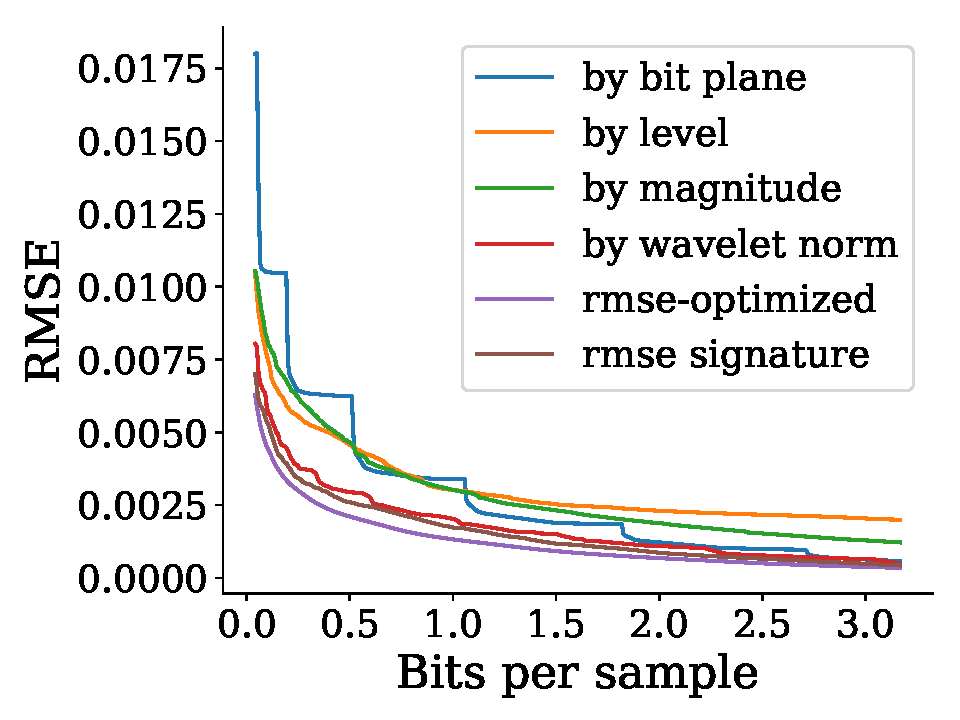
\includegraphics[width=0.48\linewidth]{rmse/rmse-optimized-boiler}}}
  \subcaptionbox{Diffusivity}{
		{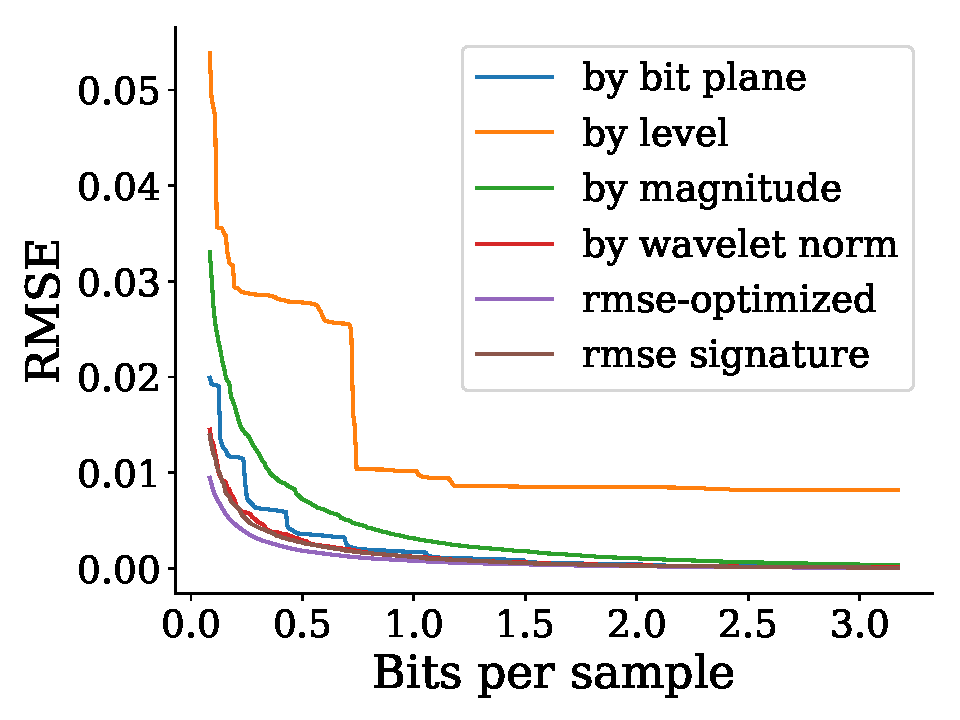
\includegraphics[width=0.48\linewidth]{rmse/rmse-optimized-diffusivity}}} 
	\subcaptionbox{Plasma}{
		{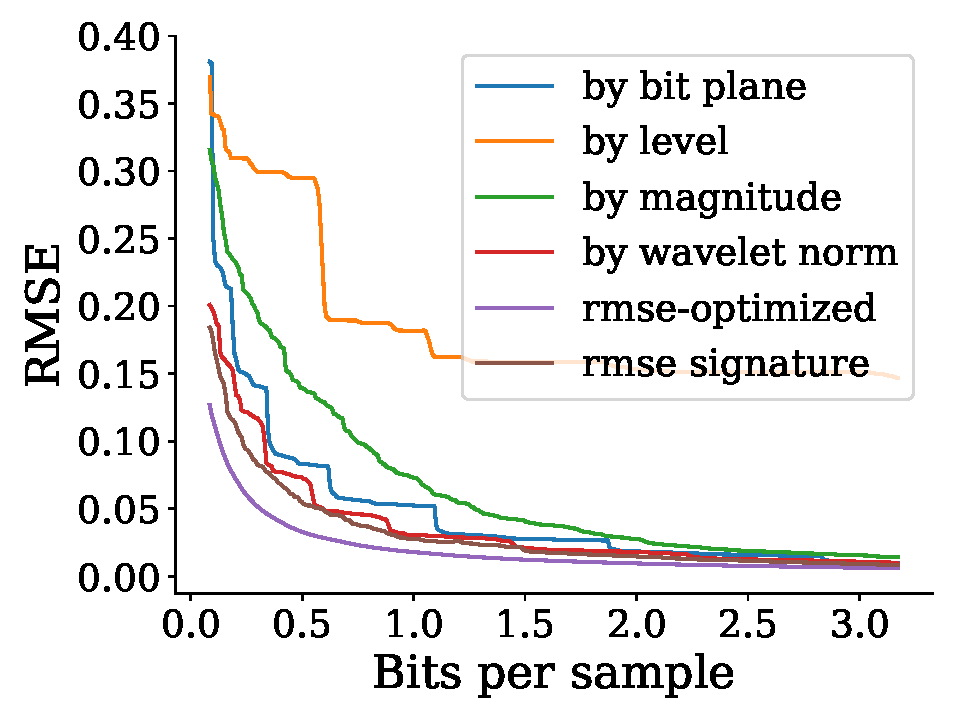
\includegraphics[width=0.48\linewidth]{rmse/rmse-optimized-plasma}}}
	\subcaptionbox{Turbulence}{
	  {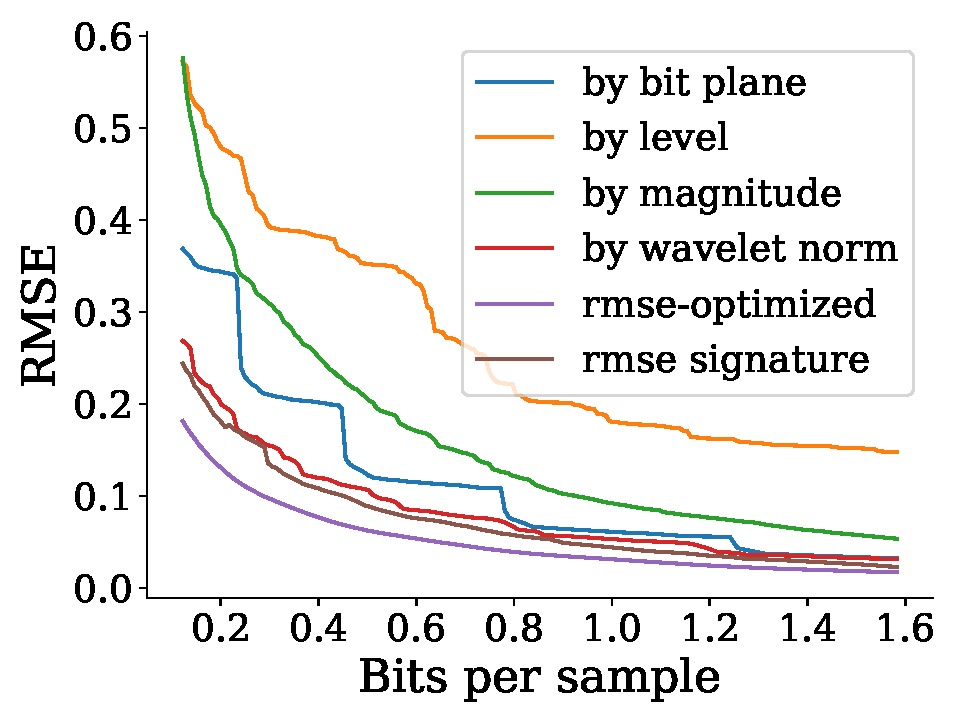
\includegraphics[width=0.48\linewidth]{rmse/rmse-optimized-turbulence}}}
  \caption{Root-mean-square error of reconstructed functions for the three data-agnostic streams
  defined in Section \ref{sec:motivation}, and the \emph{rmse-optimized} stream. Lower is better.
  The streams are truncated to highlight the differences, without omitting important information.
  \emph{rmse-optimized} performs best, followed closely by \emph{by wavelet norm}, \emph{rmse
  signature} and \emph{by bit plane}. TODO:explain any ``strange'' behavior in the
  plot.}\label{fig:rmse-optimized}
\end{figure}

\begin{figure}[h]
	\centering
	\subcaptionbox{\emph{by level}}{
	{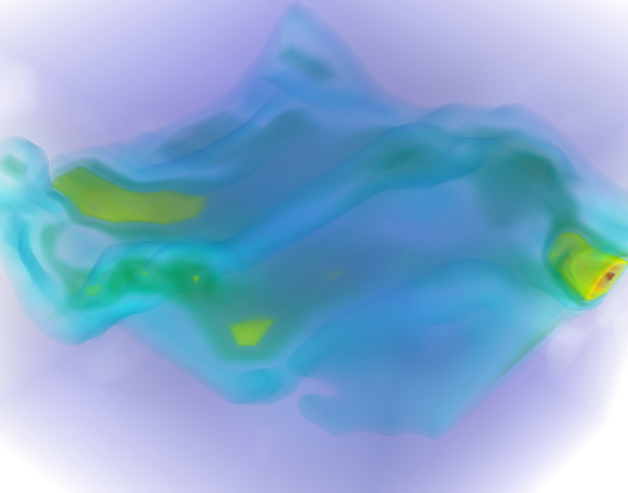
\includegraphics[width=0.31\linewidth]{rmse/rmse-plasma-level}}}
	\subcaptionbox{\emph{by bit plane}}{
	{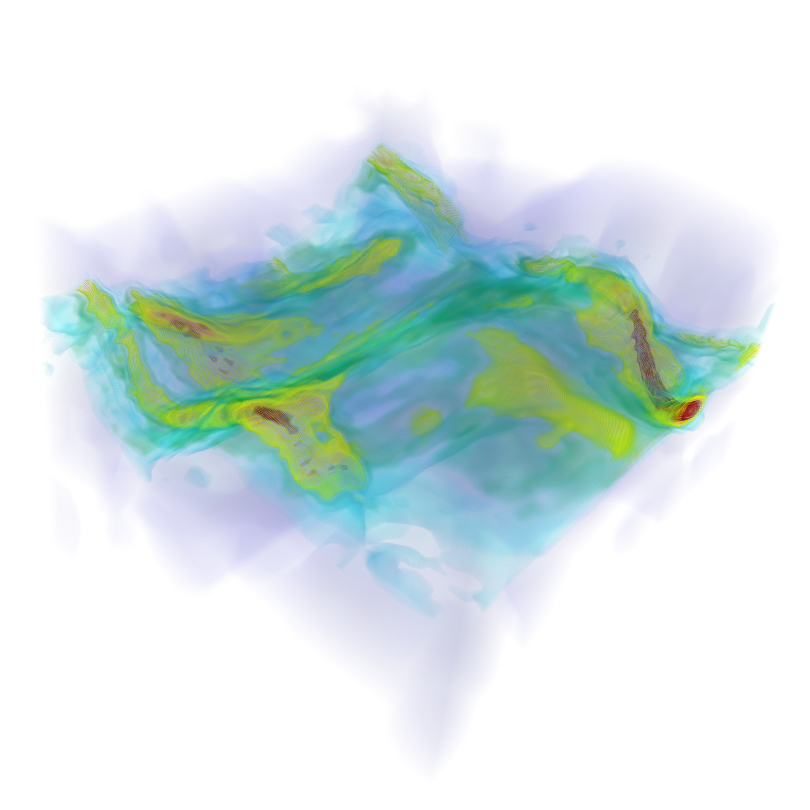
\includegraphics[width=0.31\linewidth]{rmse/rmse-plasma-bit-plane}}}
	\subcaptionbox{\emph{by magnitude}}{
	{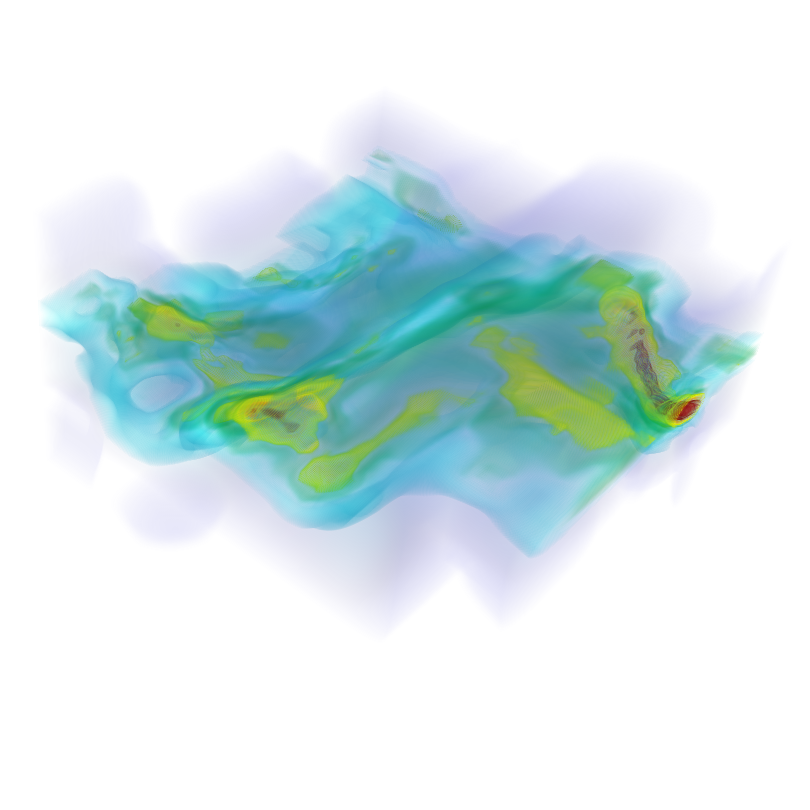
\includegraphics[width=0.31\linewidth]{rmse/rmse-plasma-magnitude}}}
	\subcaptionbox{\emph{by wavelet norm}}{
	{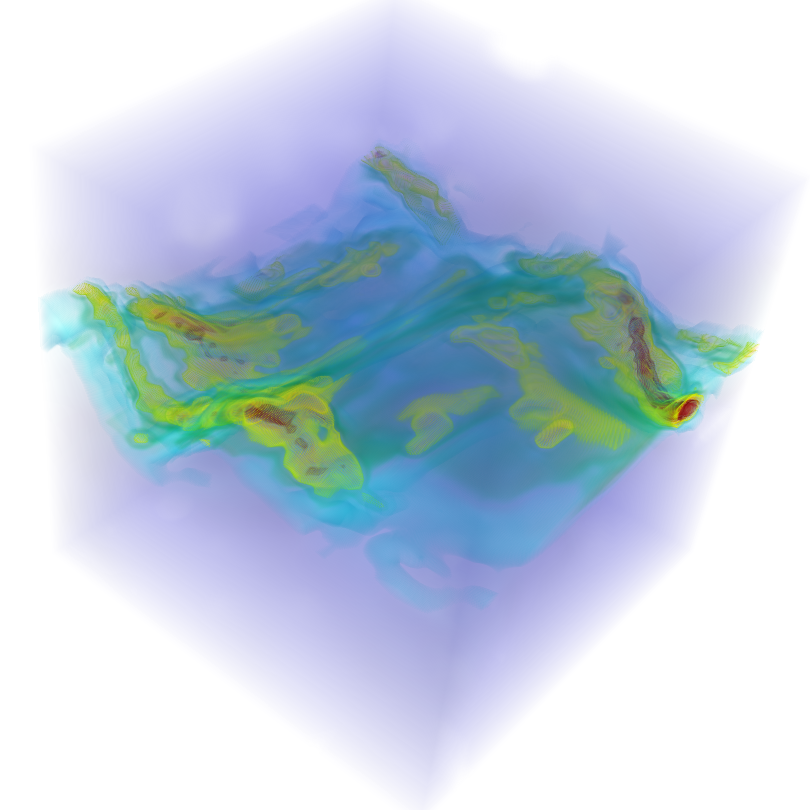
\includegraphics[width=0.31\linewidth]{rmse/rmse-plasma-wavelet-norm}}}
	\subcaptionbox{\emph{by signature}}{
	{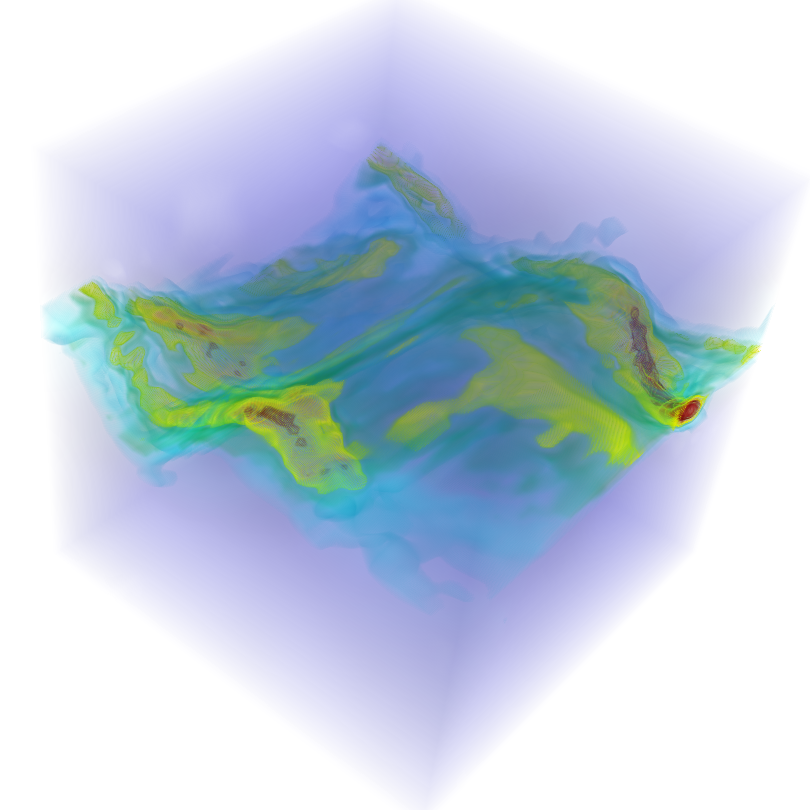
\includegraphics[width=0.31\linewidth]{rmse/rmse-plasma-signature}}}
	\subcaptionbox{\emph{groundtruth}}{
	{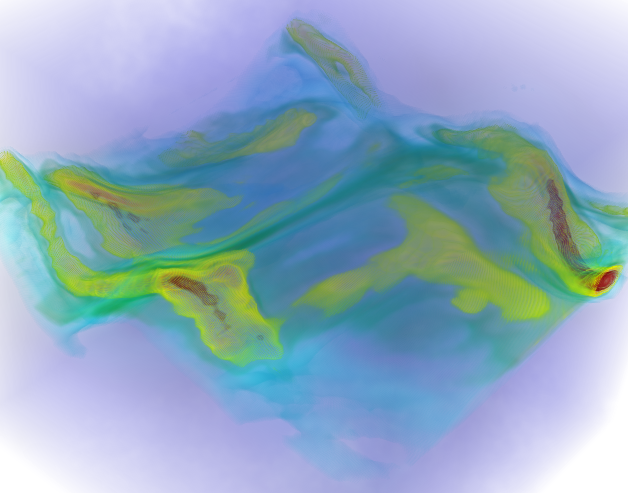
\includegraphics[width=0.31\linewidth]{rmse/rmse-plasma-groundtruth}}}
	\caption{\emph{boiler} data reconstructed at 0.03 bps}
 	\label{fig:rmse-rendering}
\end{figure}
